\documentclass[a4paper,11pt]{memoir}                                        

\usepackage[utf8]{inputenc}
\usepackage[danish]{babel}
\usepackage[T1]{fontenc}
\usepackage[left=0.8in, right=0.8in, top=1.0in, bottom=1.0in]{geometry} 
\usepackage{amsmath,amssymb}																						

% SIUnitX  http://ctan.org/pkg/siunitx
\usepackage{siunitx,booktabs}		
\sisetup{per=slash}																						
\sisetup{per-mode = reciprocal}
\sisetup{inter-unit-product = \ensuremath{{}\cdot{}}}
\sisetup{output-decimal-marker = {,} }
\DeclareSIUnit{\kroner}{kr.}

\usepackage{graphicx}
\newsubfloat{figure}% Allow subfloats in figure environment
\usepackage{dcolumn,booktabs}
\usepackage{url}
\usepackage{wrapfig}

% Redigere billed-/tabelteksterne.
\usepackage{caption}
\usepackage{subcaption}
\captionsetup{font=small,
labelfont={it,bf},textfont=sf,
format=hang}

% Packages for color handling
\usepackage[usenames,dvipsnames,svgnames,table]{xcolor}

\usepackage{threeparttable}

\usepackage[hidelinks]{hyperref}  
\hypersetup{bookmarks=false}
\hypersetup{pdftitle={Inverteret Pendul}} 
\hypersetup{pdfsubject={3. Semester Projekt, E-EEP (Elektromagnetisme, Elektronik og Projekt) og E-RMK (Regulering, Matematik og Kredsløbsteknik) E16, Grp. [4]}}
\hypersetup{pdfauthor={J\"{o}rn Jacobi, Simon Møller, Søren Frank, Nikolaj Kyed, Kenneth Petersen, Benjamin Lund}}


% TODONotes http://ctan.org/pkg/todonotes
\usepackage{todonotes}
\usepackage{placeins}

% For includering af .pdf
\usepackage{pdfpages}

% Bibliografi
\usepackage{babelbib}
\bibliographystyle{abbrv}

% Noget forsideopsætning
\usepackage{soul} % lege lege
\sodef\an{}{0.2em}{.9em plus.6em}{1em plus.1em minus.1em}
\newcommand\stext[1]{\an{\scshape#1}}

% New commands 
\newcommand{\g}{9,82 \si{\meter\per\second\squared}}
\newcommand{\dcite}[1]{\quotedblbase{#1}\textquotedblright}
\newcommand{\husk}[2]{\todo[inline,color=green!40]{#1: #2}}
\DeclareMathOperator{\lapl}{\mathcal{L}}
% Remove paragraph indentation for document
\setlength{\parindent}{0pt}
\newcommand\hcancel[2][black]{\setbox0=\hbox{$#2$}%
	\rlap{\raisebox{.45\ht0}{\textcolor{#1}{\rule{\wd0}{1pt}}}}#2} 

% Listings package
\usepackage{listings}


%Fede overskrifter
\usepackage{kpfonts}
\usepackage{calc}
\setSingleSpace{1.0}
\SingleSpacing
\definecolor{chaptercolor}{gray}{0.8}
% helper macros
\newcommand\numlifter[1]{\raisebox{-2cm}[0pt][0pt]{\smash{#1}}}
\newcommand\numindent{\kern37pt}
\newlength\chaptertitleboxheight
\makechapterstyle{hansen}{
  \renewcommand\printchaptername{\raggedleft}
  \renewcommand\printchapternum{%
    \begingroup%
    \leavevmode%
    \chapnumfont%
    \strut%
    \numlifter{\thechapter}%
    \numindent%
\endgroup%
}
  \renewcommand*{\printchapternonum}{%
    \vphantom{\begingroup%
      \leavevmode%
      \chapnumfont%
      \numlifter{\vphantom{9}}%
      \numindent%
      \endgroup}
    \afterchapternum}
  \setlength\midchapskip{0pt}
  \setlength\beforechapskip{0.5\baselineskip}
  \setlength{\afterchapskip}{1\baselineskip}
  \renewcommand\chapnumfont{%
    \fontsize{3cm}{0cm}%
    \bfseries%
    \sffamily%
    \color{chaptercolor}%
  }
  \renewcommand\chaptitlefont{%
    \normalfont%
    \huge%
    \bfseries%
    \raggedleft%
  }%
  \settototalheight\chaptertitleboxheight{%
    \parbox{\textwidth}{\chaptitlefont \strut bg\\bg\strut}}
  \renewcommand\printchaptertitle[1]{%
    \parbox[t][\chaptertitleboxheight][t]{\textwidth}{%
      %\microtypesetup{protrusion=false}% add this if you use microtype
      \chaptitlefont\strut ##1\strut}%
}}
\chapterstyle{hansen}
\aliaspagestyle{chapter}{empty} % just to save some space





\begin{document}
\begin{titlingpage}
\thispagestyle{empty}
\centering
{ \setlength{\baselineskip}{24pt}
{\Huge \stext{Inverteret Pendul} \par
%\textit{\&}\par
%\stext{Analogier}
}\par
\stext{E-EEP og E-RMK E16}
\par\vspace*{4\onelineskip}
\par

\includegraphics[width=10cm]{billeder/SDU_segl1.png}
\par\vspace*{4\onelineskip}
\stext{3. Semester Projekt}\par

\large\stext{J\"{o}rn Jacobi -- 230674}\par
\large\stext{Simon M\o ller -- 230893}\par
\large\stext{S\o ren Frank -- ddmmyy}\par
\large\stext{Nikolaj Kyed -- ddmmyy}\par
\large\stext{Kenneth Petersen -- ddmmyy}\par
\large\stext{Benjamin Lund -- ddmmyy}\par

\vfill
\vspace*{2\onelineskip}
\stext{Vejleder: Kurt B. Jessen}\par
\stext{1. september - 19. december 2016}\hfill
%\stext{24. maj 2013}\hfill
\par\vspace*{2\onelineskip}
\small
\stext{M\ae rsk Mc-Kinney M\o ller Instituttet}\par
\stext{Syddansk Universitet}
\enlargethispage{2\onelineskip}
}
\end{titlingpage}
\newpage

\renewcommand{\abstractnamefont}{\normalfont\bfseries}
\renewcommand{\abstracttextfont}{\normalfont}

\begin{abstract}
Resume her... 	
\end{abstract}

\thispagestyle{empty}

%---------- Indholdsfortegnelse  ---
\newpage
\thispagestyle{empty}
\null
\vfill
\begin{center}
\emph{Tak til, hvis nogen ...}
\end{center}
\newpage
\thispagestyle{empty}
\null

\section*{Underskrifter}
\vspace{3ex} \hfill Underskrevet d. xx/12-2016\\

\newlength{\streg} \setlength{\streg}{0.49\linewidth}
\vspace*{\fill} \rule{\streg}{1pt} \hfill \rule{\streg}{1pt}\\
\begin{minipage}[b]{\streg}
 \centering
 \rule{0pt}{4ex}
 J\"{o}rn Jacobi \\
 {\footnotesize (230674) (jojac11@student.sdu.dk)}
\end{minipage}
\hfill
\begin{minipage}[b]{\streg}
 \centering
 Simon Møller \\
 {\footnotesize (ddmmyy) (navn@student.sdu.dk)}
\end{minipage}

\vspace*{\fill} \rule{\streg}{1pt} \hfill \rule{\streg}{1pt}\\
\begin{minipage}[b]{\streg}
 \centering
 \rule{0pt}{4ex}
 Søren Frank \\
 {\footnotesize (300595) (sofra15@student.sdu.dk)}
\end{minipage}
\hfill
\begin{minipage}[b]{\streg}
 \centering
 Nikolaj Kyed \\
 {\footnotesize (ddmmyy) (navn@student.sdu.dk)}
\end{minipage}

\vspace*{\fill} \rule{\streg}{1pt} \hfill \rule{\streg}{1pt}\\
\begin{minipage}[b]{\streg}
	\centering
	\rule{0pt}{4ex}
	Kenneth Petersen \\
	{\footnotesize (ddmmyy) (navn@student.sdu.dk)}
\end{minipage}
\hfill
\begin{minipage}[b]{\streg}
	\centering
	Benjamin Lund \\
	{\footnotesize (ddmmyy) (navn@student.sdu.dk)}
\end{minipage}	
\newpage
\thispagestyle{empty}
\null
\vfill
\newpage
\tableofcontents*												
\newpage

%---------- Indledning -------------
% !TeX root = ../rapport.tex
\chapter{Indledning}

\section{Problemformulering}
At designe og fremstille et éndimensionelt vognmonteret omvendt pendul, der ved hjælp af regulering skal kunne fastholde en forudbestemt vinkel af pendulet, samt at kunne kompensere for udefrakommende påvirkninger. 

\subsection{Formål}
Formålet med projektet er, at forene de opnåede fagligheder fra undervisningen på 3. semester for elektronik og datateknik og for stærkstrøm. Alle fag fra undervisningen indgår i projektet, og er henholdsvis elektronik, elektromagnetisme, regulering, kredsløbsteknik og matematik.

\subsection{Krav til rapporten stillet i projektoplæg}
Måling og generering af elektromagnetiske felter kombineret med analog signalbehandling.
\husk{JJ}{Husk at opdatere projektoplægs krav inkl. ref. til oplæg}
\begin{itemize}
\item E-EEP (Elektromagnetisme, Elektronik og Projekt).
\item E-RMK (Regulering, Matematik og Kredsløbsteknik).
\end{itemize}

\subsection{Selvvalgte krav til produktet} \label{afs:kravspecifikation}
\begin{itemize}
\item Systemet skal kunne opretholde en maksimal svingvinkel af pendulet på 20 grader.
\item (Masser af systemet)
\item Systemet skal kunne drives af et/to batteri(er)
\item Sensoren skal være induktiv
\end{itemize}

\subsection{Problemstilling}
Følgende problemstillinger ønskes besvaret:
\begin{itemize}
\item Første
\item Anden
\end{itemize}

\subsection{Projektafgrænsning}
Følgende medtages ikke i rapporten og afgrænser projektarbejdet:
\begin{itemize}
\item Systemet skal kun virke i én retning (dimension)
\item Der ses bort fra fysisk beskrivelse af elektromotoren.
\item Der ses bort fra beskrivelsen af motorstyringen.
\item Vogn samt tilhørende motor, hjul og gearing overtages fra tidligere projekt.
\end{itemize}

\section{Løsningsmodel}
Blokdiagrammet her ?
\husk{JJ}{Del diagram af system og signalvej ?}

\section{Læsevejledning}
Rapportens læsevejledning...\\
Naturlig indførelse i emnet

\section{Arbejdsmetode}
Noter til arbejdsmetoden.
\begin{itemize}
	\item Iterativ planlægning
	\item ugentlige status møder hvor der opsummeres
	\item fleksibel opgave styring, for maksimal udnyttelse af ressourcer 
	\item To-Do lister
\end{itemize}

\section{Blokdiagram}
\begin{figure}[h!]
	\centering
	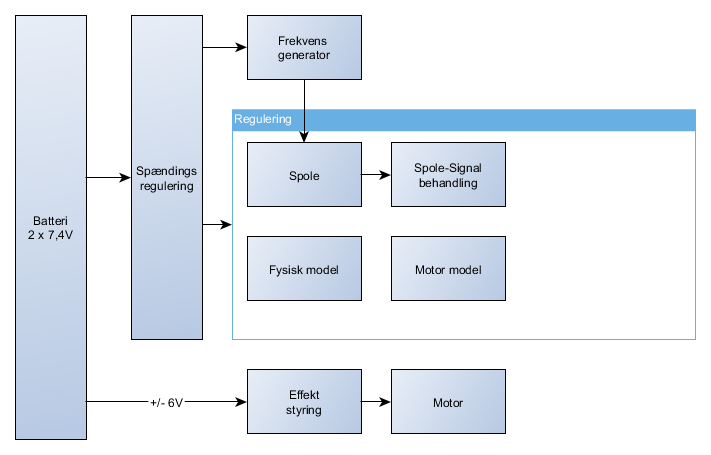
\includegraphics[width=.9\textwidth]{diagram/blokdiagram1.png}
	\caption{System blokdiagram.}
	\label{fig:blockdiagram1}
\end{figure}
\FloatBlock




							

%\listoftodos
%\newpage
\section{How To do stuff in LaTeX}

\subsection*{Figur, enkelt}
%-----------------------------------------------------------------------------
\begin{figure}[h!]
	\centering
		\includegraphics[width=.5\textwidth]{billeder/sample.png}
	\caption{Her skrives en god caption til figuren.}
	\label{fig:sample_fig_ref_her}
\end{figure}
\FloatBlock
%-----------------------------------------------------------------------------

\subsection*{Figur, dobbelt}
%-----------------------------------------------------------------------------
\begin{figure}
	\centering
	\subbottom[]{%
  		\includegraphics[width=.39\textwidth]{billeder/sample.png}
	  	\label{fig:sample_fig_ref_her_a}}
	\subbottom[]{%
		\includegraphics[width=.39\textwidth]{billeder/sample.png}
		\label{fig:sample_fig_ref_her_b}}
  	\caption{Her skrives en god caption til figuren.}
	\label{fig:sample_fig_ref_her_samlet}
\end{figure}
\FloatBlock
%-----------------------------------------------------------------------------

\subsection*{Kommentar}
%-----------------------------------------------------------------------------
\husk{Initialer}{Kommentaren skrives her}
%-----------------------------------------------------------------------------

\subsection*{Math Simple}
%-----------------------------------------------------------------------------
\begin{align}
D = \frac{1}{\Delta F}
\end{align}
%-----------------------------------------------------------------------------

\subsection*{Math uden nummer og align}
%-----------------------------------------------------------------------------
\begin{align}
D &= \frac{1}{\Delta F} \Rightarrow \nonumber \\
\Omega &= \mathrm{Noget helt andet}
\end{align}
%-----------------------------------------------------------------------------
\subsection*{Tabeller med caption}
\begin{table}
\centering
    \caption{Konstanter som bruges i overstående formler.}
\label{tab:konst1}
    \begin{tabular}{ | l | l |}
    \hline
    A & 18 [V] \\ \hline
    f & 50 [Hz]  \\ \hline
    T & 20 [s]  \\ \hline
    $\omega$ & 30 \\ \hline
    k & 100 \\ \hline
    \end{tabular}
    \end{table}

\newpage

%---------- Chapter ----------------
\chapter{Chapter}\label{kap:chap1}

%---------- Parts ----------------
\section{Section}\label{sec:sect1}

%---------- Chapter ----------------
\chapter{Diskussion og vurdering}\label{kap:diskussion}
Som helhed virkede de fleste af tilgangene for at løfte opgaven tilfredsstillende.
Arbejdsmetoder og workflow viste sig at fungere som forventet.
Planlægning med stramme deadline blev overholdt, og gav anledning til overblik i projektet.

I følgende afsnit vil en mere dybdegående diskussion og vurdering gennemgås med relation til de enkelte afsnit. 

\subsection{Fysisk model}
Ved at anvende klassisk fritlegeme analyse af pendulet lykkedes det at få en reguleringsmæssig brugbar beskrivelse af fysikken. 
Det var dog en lang og besværlig vej at løse problemet på, da man med anden viden, fx Lagrange og statespace analyse ville frembringe et brugbart resultat.
Der blev anvendt en del tilnærmelser i udledningen. 
Da alle tilnærmelser er velargumenteret, vurderes det at deres anvendelse er valide og det endelige resultat anses for korrekt.   

\subsection{Vognens overførelsesfunktioner}
Da hele vognen med pendul og motor var arvet fra en tidligere projekt gruppe, var en af udfordringerne at finde frem til den dynamik der beskriver disse dele.
Den anvendt metode viste sig at fungere og det endelige resultat kunne, ud fra en velovervejet simplificering, anvendes i den samlede systembeskrivelse der ligger til grund for bestemmelsen af regulatoren.
Til fremtidige forbedringer ville udskiftning af fx motor kunne føre til en mere dybdegående beskrivelse af systemets overførelsesfunktion, og derved give en endnu bedre regulering og stabilitet.

\subsection{Sensor}
Ud fra analysering af sammenkoblingen mellem to solenoider, lykkedes det vha. forskellige teorier - heriblandt Faradays lov - at lave en velfungerende model af et sensorsystem. 
Det mest krævende var, at lave et præcist resultat for magnetfeltet, da dette krævede flere teknikker, heriblandt mange matematiske udledninger.
Faktorerne for den inducerede afsenderspole, var meget diskuteret, da strømmen fra frekvensgeneratoren afhang af styrken på magnetfeltet denne dannede - herudover også trådtykkelse og længde. 
Da alle teoretiske beregninger blev eftervist i laboratoriet, antages der med nogen tilnærmelse, at de endelige resultater kan antages for korrekte.\\
Under designet af CAD-tegningerne var det en udfordring at lave et system med nem montering på den arvede vogn. Efter nogle 3D-print forsøg og adskillige målinger lykkedes det at lave et godt brugbart system som var nemt at montere, samt nemt at vikle spoler på. Derudover gav det køretøjet et nogenlunde stilrent udseende, pga. print-monteringspladen og batteri-hus kombinationen.\\
Til dimensionering af timer-kredsen, blev der anvendt vedlagte ligninger i databladet.
Det var herfra muligt at dimensionere komponentstørrelser, der ville lave et signal med en frekvens, der lå tæt på den ønskede.
Desværre viste målinger på kredsløbet, at frekvensen varierede mere på det endelige produkt, end ved breadboard prototypen.
Dette blev først opdaget hen mod slutning af projektet, så fejlfinding ikke var mulig, men fejlen skyldes højst sandsynligt en forkert komponent.
Endvidere viste det sig, at udgangssignalet ikke oscillerede mellem en konstant positiv og negativ spænding af samme størrelse, hvor årsagen til dette er endnu ikke kendt.
En mulig forbedring kunne være at designe en frekvensgenerator baseret på en anden topologi.

\subsection{Signalbehandling}
Ud fra løbende test af hvert kredsløb på breadboards, blev de endelige kredsløb dimensioneret.
På trods af støj i breadboards, virkede kredsløbene efter hensigten.
For at undgå støj i de endelige kredsløb, blev der tilføjet afkoblingskondensatorer, hvor det var muligt.
En mulig forbedring af signalbehandlingen blev undersøgt, hvor der blandt andet blev kigget på en aktiv ensretter kreds. Problemet med denne var dog, at der skulle bruges to operationsforstærkere til én ensretter.
Det endelige kredsløb indeholder to aktiv båndpas filtre, hvilket kunne viste sig at være en god idé, da disse ikke har særlig stor impedans påvirkning af de omkringliggende kredsløb.
Grundet approksimering af komponentværdier til E12 og E6 serien, kom der afvigelser fra de teoretiske forventninger.

\subsection{Motorstyring}
Det viste sig tilstrækkeligt at anvende bi-directional DC-motor driver topologi som styring af motoren. 
Den negative feedback sørgede for en velfungerende regulering af strømmen igennem motoren, som var vigtig for at reguleringssystemet kunne fungere og give den ønskede stabilitet.
Kompleksiteten omkring motoren var stor, så derfor var mange tilnærmelser nødvendige.
Disse tilnærmelser anses dog for at være velbegrundede, men om deres omfang var dækkende, vides dog ikke med sikkerhed.
Under projektarbejdet, viste en manglende strøm igennem motoren at være et problem mht. respons hastigheden af vognen overfor udefrakommende forstyrrelser.     
En ændring af design, der ved indførelse af en ekstra $\pm 9 \si{\volt}dc$ forsyning til motorstyringens operationsforstærker, blev løst.
Det ville på sigt, give en bedre stabilitet at udskifte den nuværende motorstyring, med en der kan håndtere mere effekt, men siden den nuværende motoreffekt giver anledning til mistet vejgreb fra hjul til underlag, vil en opgradering af hjul være et bedre valg. 

\subsection{Regulering}
Opstilling af det samlede reguleringssystem viste sig at være en stor og kompleks opgave.
Der var mange del overførelsesfunktioner der ikke blot skulle beskrives, men det var også nødvendigt at identificere hvilke simplificeringer og lineariseringer der var mulige at lave, uden at miste den nødvendige information i åben-løkke beskrivelsen af reguleringssløjfe.
Valget af P-lead kompensator som regulator viste sige at være tilstrækkeligt og gav den nødvendige fasemargin der skulle til for at stabilisere pendulet.
Det viste sig svært at få målt systemets overførelsesfunktion, men med lidt god vilje ligger målingen rimelig tæt på den teoretiske model. 



							

%---------- Chapter ----------------
\chapter{Konklusion} \label{kap:konklusion}
En klassisk modelfremstilling af det fysiske system kunne give den nødvendige model til at beskrive det inverterede pendul.
Det viste sig muligt, at ved måling og beregninger, at bestemme dynamikken for vogn og motor.
Sammen med overførelsesfunktionerne fra de elektriske kredse i systemet, var det muligt at danne et samlet reguleringssystem og ved klassisk reguleringsteori at fremstille og dimensionere en P-lead regulator, der kunne stabilisere systemet.
Det blev vist at pendulets vinkel kan bestemmes, ved at anvende elektromagnetiske felter frembragt af spoler, hvor der blev opstillet en tilnærmet teoretisk model, der kunne eftervises.
Det blev også eftervist, hvordan magnetiske felter kobler sig imellem 2 spoler.
I det elektriske kredsløb viste en signalbehandling i form af et filter, en ensretning og signalsammenligning sig tilstrækkeligt for at kunne bruge transducerens signal til regulering.
Den valgte motorstyring blev designet så vognen kunne bevæge sig efter hensigten.
Den nødvendige forsyning, til de enkelte kredsløb, kunne med en spændingsregulator og en shunt-regulator realiseres.
Alle nødvendige konstruktionsdele til vognen, kunne med fordel fremstilles ved CAM og 3D-printer teknologi.

Det kan derfor konkluderes at alle punkterne i problemstillingen er blevet besvaret, at det udarbejdede produkt er funktionelt samt overholder de stillede krav for projektet. 							

\nocite{*}
\bibliography{rapport}\label{bilag:litteratur}
%\listoffigures
%\listoftables

%--------- Bilag -------------------
\appendix
%\input{section/small_model}																
%\input{section/udstyr}
%\input{section/ugeplan}
%\newpage
\section{Oversigt af CD}\label{bilag:cd}
Oversigt af indholdet på den medfølgende cd. Beskrivelsen dækker kun det første mappeniveau og de underliggende filer kan fremstå i forskellig kvalitet og formater. Fodnoterne henviser til den nødvendige software, der skal bruges for at åbne filerne.

\begin{table}[h!]
\centering
\caption{Mappeoversigt af rapport CD}
\label{tab:ordliste}
\begin{threeparttable}
\begin{tabular}{l l}
\toprule
\multicolumn{1}{l}{Mappe}       &
\multicolumn{1}{l}{Beskrivelse}  \\ 
\midrule
Mappe					& Beskrivelse \\
\bottomrule
\end{tabular}
\begin{tablenotes}
\item[a] fodnote til mappe  \url{http://sdu.dk}
\end{tablenotes}
\end{threeparttable}
\end{table}


%\chapter{Styklister} \label{bilag:styklister}
\husk{JJ}{Styklister med ref til alle diagrammer}

\begin{table}[h!]
\small
\centering
\caption{Stykliste for diagram xxx}
\label{tab:udstyr}
\begin{threeparttable}
\begin{tabular}{ l l l l l l l }
\toprule
\multicolumn{1}{l}{\textbf{Komp.}}       &
\multicolumn{1}{l}{\textbf{Værdi}}       &
\multicolumn{1}{l}{\textbf{Type}}       &
\multicolumn{1}{l}{\textbf{Tol.}} &
\multicolumn{1}{l}{\textbf{Klasse}} &
\multicolumn{1}{l}{\textbf{Bemærkning}} &
\multicolumn{1}{l}{\textbf{Type / Lev.}}  \\ 
\hline
R1,R2 & $\SI{68}{\ohm}$			& Keramisk	SMD	& $\pm 1\%$ 		 & $\SI{0.25}{\watt}$	  & 100ppm/\si{\celsius}  & RC12 0805, Phycomp \\
R3 & $\SI{10}{\kilo\ohm}$		& Keramisk	SMD	& $\pm 1\%$ 		 & $\SI{0.25}{\watt}$	  & 100ppm/\si{\celsius}  & RC12 0805, Phycomp \\
R4 & $\SI{1}{\kilo\ohm}$		& Keramisk	SMD	& $\pm 1\%$ 		 & $\SI{0.25}{\watt}$	  & 100ppm/\si{\celsius}  & RC12 0805, Phycomp \\
R5 & $\SI{680}{\ohm}$			& Keramisk	SMD	& $\pm 1\%$ 		 & $\SI{0.25}{\watt}$	  & 100ppm/\si{\celsius}  & RC12 0805, Phycomp \\
R6 & $\SI{15}{\kilo\ohm}$		& Keramisk	SMD	& $\pm 1\%$ 		 & $\SI{0.25}{\watt}$	  & 100ppm/\si{\celsius}  & RC12 0805, Phycomp \\
R7,R17 & $\SI{1}{\kilo\ohm}$		& Potentiometer		& $\pm 10\%$ 		 & $\SI{0.5}{\watt}$	  & 100ppm/\si{\celsius}  & 3296 Square Trimpot, Bourns  \\
R8,R13 & $\SI{6.8}{\kilo\ohm}$		& Keramisk	SMD	& $\pm 1\%$ 		 & $\SI{0.25}{\watt}$	  & 100ppm/\si{\celsius}  & RC12 0805, Phycomp \\
R9,R14 & $\SI{1.5}{\kilo\ohm}$		& Keramisk	SMD	& $\pm 1\%$ 		 & $\SI{0.25}{\watt}$	  & 100ppm/\si{\celsius}  & RC12 0805, Phycomp \\
R10,R15 & $\SI{47}{\kilo\ohm}$		& Keramisk	SMD	& $\pm 1\%$ 		 & $\SI{0.25}{\watt}$	  & 100ppm/\si{\celsius}  & RC12 0805, Phycomp \\
R11,R12,R16 & $\SI{4.7}{\kilo\ohm}$		& Keramisk	SMD	& $\pm 1\%$ 		 & $\SI{0.25}{\watt}$	  & 100ppm/\si{\celsius}  & RC12 0805, Phycomp \\
R18 & $\SI{1.5}{\kilo\ohm}$		& Metalfilm	& $\pm 1\%$ 		 & $\SI{0.6}{\watt}$	  & 50ppm/\si{\celsius}  & MRS25, Philips \\
R40 & $\SI{15}{\kilo\ohm}$ 	& Keramisk SMD 	& $\pm 1\%$			& $\SI{0.25}{\watt}$ 	& 100ppm/\si{\celsius}	& RC12 1206, Phycomp \\
R41 & $\SI{1}{\kilo\ohm}$ 	& Keramisk SMD 	& $\pm 1\%$			& $\SI{0.25}{\watt}$ 	& 100ppm/\si{\celsius}	& RC12 1206, Phycomp \\
R42 & $\SI{330}{\kilo\ohm}$ 	& Keramisk SMD 	& $\pm 1\%$			& $\SI{0.25}{\watt}$ 	& 100ppm/\si{\celsius}	& RC12 1206, Phycomp \\
C1,C2,C4,C6,C20, C40 & $\SI{10}{\micro\farad}$ & Keramisk SMD & $\pm 10\%$ & 50 \si{\volt}  & 15ppm/\si{\celsius} & X7R-serie 1206, Phycomp \\
C3,C5,C12,C13,C14,C15,C18,C19,C21,C22, C41,C42 & $\SI{100}{\nano\farad}$ & Keramisk SMD & $\pm 10\%$ & 50 \si{\volt} & 15ppm/\si{\celsius} & X7R-serie 1206, Phycomp \\
C7 & $\SI{1}{\nano\farad}$ & Keramisk SMD & $\pm 5\%$ & 50 \si{\volt} & 30ppm/\si{\celsius} & NP0-serie 1206, Phycomp \\
C8 & $\SI{10}{\nano\farad}$ & Keramisk SMD & $\pm 5\%$ & 50 \si{\volt} & 30ppm/\si{\celsius} & NP0-serie 0805, Phycomp \\
C9 & $\SI{1}{\micro\farad}$ & Keramisk SMD & $\pm 10\%$ & 50 \si{\volt} & 15ppm/\si{\celsius} & X7R-serie 0805, Phycomp \\
C10,C11,C16,C17 & $\SI{470}{\pico\farad}$ & Keramisk SMD & $\pm 10\%$ & 50 \si{\volt} & 15ppm/\si{\celsius} & X7R-serie 0805, Phycomp \\
D1,D2 & BZX79C6V2 & Zener diode & $\pm 5 \%$ & \SI{0.5}{\watt} & \SI{4}{\milli\watt\per\celsius} & Fairchild Semiconductor \\
D3,D4 & 1N4148 & Ensretter diode & N/A & \SI{0.5}{\watt} & \SI{5}{\milli\watt\per\celsius} & Fairchild Semiconductor \\
D5 & LED grøn 3mm & Grøn lysdiode & N/A & \SI{0.1}{\watt} & N/A & Ukendt \\
IC1 & NE555P & Timerkreds SMD & $V_{cc}= 18 \si{\volt}$ & N/A & 50ppm/\si{\celsius} & Texas Instruments \\
IC2,IC3,IC40 & TL071P & Op. Amp SMD & $V_{cc}=\pm 18 \si{\volt}$ & N/A & \SI{18}{\micro\volt\per\celsius} & Texas Instruments \\
IC4 & AD623AN & Op. Amp SMD & $V_{cc} = 12 \si{\volt}$ & \SI{650}{\milli\watt} & 50ppm/\si{\celsius} & Analog Devices \\
IC5 & LM317T & Spændingsregulator & $V_{o} , V_{i} = 40 \si{\volt}$ & \SI{20}{\watt} & $i_{max} = 1.5 \si{\ampere}$ & Motorola \\
SW1 & 6-polet knap & N/A & N/A & N/A & N/A & Shadow \\

\hline
\bottomrule
\end{tabular}
%\begin{tablenotes}
%\item[a] \textit{Maximum værdi fra datablad}
%\item[b] \textit{Anslået værdi baseret på generelle datablade}
%\end{tablenotes}
\end{threeparttable}
\end{table} 
%\input{section/diagram}


\end{document}